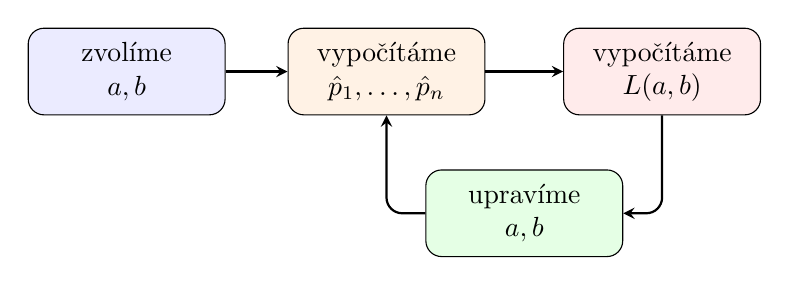
\begin{tikzpicture}[
    >=stealth,
    box/.style={
        draw,
        rounded corners=2mm,
        minimum width=25mm,
        minimum height=11mm,
        align=center
    },
    arr/.style={
        ->,
        thick,
        rounded corners=2mm
    }
]
    \node[box, fill=blue!8] (parameters) at (0,0)
        {zvolíme\\\(a,b\)};

    \node[box, fill=orange!10] (outputs) at (3.3,0)
        {vypočítáme\\
        \(\hat p_1,\ldots,\hat p_n\)};

    \node[box, fill=red!8] (loss) at (6.8,0)
        {vypočítáme\\\(L(a,b)\)};

    \node[box, fill=green!10] (change) at (5.05,-1.8)
        {upravíme\\\(a,b\)};

    % Pomocné body pro pravoúhlé šipky
    \coordinate (rightturn) at (6.8,-1.8);
    \coordinate (leftturn) at (3.3,-1.8);

    \draw[arr]
        (parameters.east) -- (outputs.west);

    \draw[arr]
        (outputs.east) -- (loss.west);

    \draw[arr]
        (loss.south) --
        (rightturn) --
        (change.east);

    \draw[arr]
        (change.west) --
        (leftturn) --
        (outputs.south);
\end{tikzpicture}
